\documentclass[11pt,a4paper]{ctexart}
\usepackage[a4paper,margin=1.72cm]{geometry}
\usepackage{amsmath,amssymb,mathtools}
\usepackage{booktabs,tabularx,longtable,array,multirow}
\usepackage{enumitem}
\usepackage{tikz}
\usetikzlibrary{arrows.meta,positioning,shapes.geometric,fit,calc,matrix,decorations.pathreplacing}
\usepackage[most]{tcolorbox}
\usepackage{xcolor}
\usepackage{fancyhdr}
\usepackage{hyperref}
\usepackage{microtype}
\usepackage{listings}
\usepackage{pifont}
\usepackage[hypcap=false]{caption}
\setlength{\parindent}{2em}
\setlength{\parskip}{0.30em}
\setlist[itemize]{itemsep=0.16em,topsep=0.26em}
\setlist[enumerate]{itemsep=0.16em,topsep=0.26em}
\hypersetup{colorlinks=true,linkcolor=blue!45!black,urlcolor=blue!50!black}

\definecolor{mainblue}{RGB}{45,86,140}
\definecolor{deepblue}{RGB}{30,62,102}
\definecolor{softblue}{RGB}{238,245,252}
\definecolor{softgreen}{RGB}{238,249,243}
\definecolor{softorange}{RGB}{253,246,233}
\definecolor{softred}{RGB}{253,239,239}
\definecolor{softgray}{RGB}{246,247,249}
\definecolor{deepgreen}{RGB}{35,105,75}
\definecolor{deeporange}{RGB}{165,98,22}
\definecolor{deepred}{RGB}{150,55,55}
\definecolor{purple}{RGB}{94,66,140}
\definecolor{softpurple}{RGB}{245,241,251}
\definecolor{teal}{RGB}{38,112,115}
\definecolor{softteal}{RGB}{238,248,248}
\definecolor{gold}{RGB}{156,120,28}
\definecolor{softgold}{RGB}{252,249,235}

\pagestyle{fancy}
\fancyhf{}
\lhead{408 OS 专题}
\rhead{文件系统：名称、对象、索引与持久化}
\cfoot{\thepage}
\renewcommand{\headrulewidth}{0.4pt}
\setlength{\headheight}{14pt}

\newtcolorbox{corebox}[1][]{colback=softblue,colframe=mainblue,title=#1,fonttitle=\bfseries,boxrule=0.8pt,arc=2mm}
\newtcolorbox{exam}[1][]{colback=softorange,colframe=deeporange,title=#1,fonttitle=\bfseries,boxrule=0.8pt,arc=2mm}
\newtcolorbox{warn}[1][]{colback=softred,colframe=deepred,title=#1,fonttitle=\bfseries,boxrule=0.8pt,arc=2mm}
\newtcolorbox{eng}[1][]{colback=softgreen,colframe=deepgreen,title=#1,fonttitle=\bfseries,boxrule=0.8pt,arc=2mm}
\newtcolorbox{method}[1][]{colback=softgray,colframe=black!45,title=#1,fonttitle=\bfseries,boxrule=0.6pt,arc=2mm}
\newtcolorbox{bridge}[1][]{colback=softpurple,colframe=purple,title=#1,fonttitle=\bfseries,boxrule=0.8pt,arc=2mm}
\newtcolorbox{statebox}[1][]{colback=softteal,colframe=teal,title=#1,fonttitle=\bfseries,boxrule=0.8pt,arc=2mm}
\newtcolorbox{history}[1][]{colback=softgold,colframe=gold,title=#1,fonttitle=\bfseries,boxrule=0.8pt,arc=2mm}

\newcommand{\kw}[1]{\textbf{#1}}
\newcommand{\code}[1]{\texttt{\detokenize{#1}}}
\newcommand{\arr}{\;\longrightarrow\;}
\newcommand{\yes}{\textcolor{deepgreen}{\ding{51}}}
\newcommand{\no}{\textcolor{deepred}{\ding{55}}}

% ---- Unified figure grammar ----
\tikzset{
  fsnode/.style={draw=mainblue,rounded corners=1.6mm,minimum width=2.60cm,minimum height=0.95cm,
    align=center,inner sep=3pt,font=\small,fill=softblue},
  fsnodeg/.style={fsnode,draw=deepgreen,fill=softgreen},
  fsnodeo/.style={fsnode,draw=deeporange,fill=softorange},
  fsnodep/.style={fsnode,draw=purple,fill=softpurple},
  fsnodegray/.style={fsnode,draw=black!45,fill=softgray},
  persist/.style={draw=deeporange,double,rounded corners=1.2mm,minimum width=2.60cm,minimum height=0.95cm,
    align=center,inner sep=3pt,font=\small,fill=softorange},
  mainflow/.style={-{Latex[length=2mm]},line width=0.8pt,draw=deepblue},
  refedge/.style={-{Latex[length=1.8mm]},densely dashed,line width=0.7pt,draw=purple},
  optedge/.style={-{Latex[length=1.8mm]},dotted,line width=0.8pt,draw=teal},
  crossout/.style={line width=1.2pt,draw=deepred},
  labelnote/.style={font=\scriptsize,fill=white,inner sep=1.2pt,text=black!75}
}

\lstset{
  basicstyle=\ttfamily\small,
  columns=fullflexible,
  frame=single,
  rulecolor=\color{black!25},
  breaklines=true,
  showstringspaces=false,
  aboveskip=0.6em,
  belowskip=0.6em
}

\title{\vspace{-1.2cm}\textbf{文件系统：名称、对象、索引与持久化}\\[0.35em]
\large 从路径、fd、inode、块映射到页缓存、日志与崩溃一致性}
\author{408 专题手册 · 操作系统文件系统篇}
\date{}

\begin{document}
\maketitle

\begin{corebox}[核心模型：文件系统建立持久对象世界]
文件系统在块式持久存储之上，为程序制造一个看起来拥有\kw{名字、对象、层次、共享、保护、随机访问与长期存在}的世界。

分析主线：
\[
\boxed{\begin{aligned}
\text{Name}\arr\text{Object}\arr\text{Open State}\arr\text{Byte Range}\\
\arr\text{Cached Page}\arr\text{Block Mapping}\arr\text{Persistent State}
\end{aligned}}
\]

横向始终检查三个约束：
\[
\boxed{\text{Protection}}\qquad
\boxed{\text{Lifecycle}}\qquad
\boxed{\text{Crash Consistency}}
\]

学生版一句话：\kw{先找到“谁”，再建立访问关系，再找到“哪一段数据”，最后保证它即使掉电也仍然是一个合法文件。}
\end{corebox}

\begin{eng}[系统的通用推理：崩溃一致性（Crash Consistency）中的元数据不变量]
在文件系统持久化与崩溃恢复中，同样遵循 OS 通用系统推理引擎（OS System Reasoning Engine）：
\[
\text{State (Bitmap/Inode/Data Blocks)}
\to\text{Crash/Power Fault (突发断电)}
\to\text{Failure (块被重复分配/孤立)}
\to\text{Invariant (Bitmap Free } \iff \text{无 Inode 占用)}
\]
为了拦截这类毁坏性坏状态，文件系统引入了\kw{预写日志（Journaling / WAL）}或\kw{写顺序约束（Write-Ordering）}作为最小机制，确保磁盘元数据在故障恢复后依然满足逻辑一致性。
\end{eng}

\tableofcontents
\newpage

\section{第 0 章：文件系统究竟解决什么问题}

\subsection{从裸块设备到“文件世界”}
假设底层只给你一串可以读写的编号块：
\[
B_0,B_1,B_2,\ldots,B_{N-1}.
\]
单靠这些块，应用无法自然回答：
\begin{itemize}
  \item 这堆字节叫什么名字？目录层次在哪里？
  \item 这段数据属于哪个逻辑对象？对象有多大、谁拥有、谁能读写？
  \item 文件增长以后，新块从哪里来？删除以后空间怎样回收？
  \item 多个名字、多个进程能否指向同一对象？
  \item 内存缓存和磁盘状态不同步时，什么叫“写成功”？
  \item 创建文件需要改多个磁盘结构，掉电发生在中间怎么办？
\end{itemize}

因此文件系统至少提供四个承诺：
\begin{center}
\small
\begin{tabularx}{\linewidth}{>{\bfseries}p{0.19\linewidth} X X}
\toprule
承诺 & 对应用提供的幻觉/抽象 & 内核必须解决的问题 \\
\midrule
Naming & 用路径而不是块号找对象 & 目录、路径解析、mount、链接 \\
Object & 把字节组织成“文件” & inode/FCB、元数据、权限 \\
Access & 打开后可持续读写 & fd、打开文件描述（OFD）、offset \\
Persistence & 重启后对象仍可解释 & layout、分配、写回、日志、恢复 \\
\bottomrule
\end{tabularx}
\end{center}

\begin{bridge}[文件系统与前面专题的边界]
\begin{itemize}
  \item \kw{I/O 专题}回答：已经知道要访问哪个块以后，请求如何提交、DMA 如何搬运、设备如何完成、进程如何被唤醒。
  \item \kw{虚拟内存专题}回答：虚拟页怎样映射到物理页；\code{mmap()} 时文件页怎样成为虚拟地址的后备对象。
  \item \kw{文件系统专题}回答：\code{/a/b/c} 或 \code{fd=3} 怎样变成文件对象、文件偏移与存储位置，以及这些持久元数据怎样保持一致。
\end{itemize}
\end{bridge}

\subsection{五层映射 + 一个持久化约束}
\begin{center}
\begin{tikzpicture}[x=3.15cm,y=1.85cm]
  \node[fsnode] (name) at (0,0) {Name\\[-1pt]\scriptsize path/component};
  \node[fsnode] (obj) at (1,0) {Object\\[-1pt]\scriptsize inode/FCB};
  \node[fsnode] (open) at (2,0) {Open State\\[-1pt]\scriptsize fd/OFD/offset};
  \node[fsnode] (byte) at (3,0) {Byte Range\\[-1pt]\scriptsize offset/LBN};
  \node[fsnodeg] (cache) at (3,-1) {Cached Page\\[-1pt]\scriptsize 页缓存};
  \node[fsnodeo] (map) at (2,-1) {Block Mapping\\[-1pt]\scriptsize index/extent};
  \node[persist] (disk) at (1,-1) {Persistent State\\[-1pt]\scriptsize metadata+data};
  \node[fsnodep] (life) at (0,-1) {Lifecycle\\[-1pt]\scriptsize link/open refs};
  \draw[mainflow] (name) -- (obj);
  \draw[mainflow] (obj) -- (open);
  \draw[mainflow] (open) -- (byte);
  \draw[mainflow] (byte) -- (cache);
  \draw[mainflow] (cache) -- (map);
  \draw[mainflow] (map) -- (disk);
  \draw[refedge] (obj) -- (life);
  \draw[refedge] (life) -- (disk);
\end{tikzpicture}
\end{center}

\begin{method}[文件系统六问]
以后任何文件系统机制，都先问：
\begin{enumerate}
  \item 名字怎样找到对象？
  \item 进程怎样在打开以后持续引用对象？
  \item 文件中的字节位置怎样找到逻辑块/页？
  \item 逻辑块怎样找到持久存储位置？
  \item 新空间怎样分配、旧空间怎样回收？
  \item 高层操作由多次持久写组成时，怎样抵抗崩溃？
\end{enumerate}
\end{method}

\section{Part I：名字怎样找到对象}

\section{第 1 章：文件抽象、元数据与对象身份}

\subsection{文件不是“磁盘上一段连续字节”}
从应用角度，普通文件最稳定的抽象通常是\kw{一个可按字节定位的持久对象}。它同时拥有：
\begin{itemize}
  \item 内容（data）；
  \item 大小、权限、所有者、时间戳等元数据（metadata）；
  \item 在特定文件系统中的对象身份；
  \item 将逻辑位置映射到存储空间的方法。
\end{itemize}

\begin{corebox}[元数据与数据分离]
UNIX/inode 思想的关键不是“inode 这个单词”，而是把\kw{对象身份与元数据}从\kw{名字}和\kw{数据内容}中拆开：
\[
\boxed{\text{Name}\neq\text{Object}\neq\text{Data}}
\]
文件名属于命名空间；inode/FCB 描述对象；数据块保存内容。正因为三者解耦，硬链接、rename、权限修改与共享才有清晰语义。
\end{corebox}

\subsection{FCB、inode 与“文件名在哪”}
\begin{center}
\small
\begin{tabularx}{\linewidth}{>{\bfseries}p{0.20\linewidth} X X}
\toprule
概念 & 408 稳定理解 & UNIX/Linux 典型映射 \\
\midrule
FCB & 描述文件的控制信息/元数据的抽象 & inode 可看作一种具体 FCB 风格实现 \\
inode & 对象元数据 + 数据定位信息，\kw{不以文件名作为身份} & 磁盘 inode 与内存 inode object \\
Directory Entry & 把目录中的一个名字映射到对象标识 & 经典 inode FS 中常是 name $\to$ inode number \\
\bottomrule
\end{tabularx}
\end{center}

\begin{warn}[dentry 不能与“磁盘目录项”混成一个东西]
408 中的\kw{目录项}通常指持久目录文件里的记录；Linux VFS 的 \code{struct dentry} 是\kw{内存中的路径组件/名称缓存对象}。Linux VFS 文档明确说明 dentry 存在于 RAM、用于 pathname lookup，不保存到磁盘。正式做题时先判断题目说的是“目录文件里的 entry”还是“VFS dentry”。
\end{warn}

\subsection{文件逻辑结构与访问方式}
408 常把逻辑结构分为：
\begin{itemize}
  \item \kw{无结构字节流}：应用自己解释内容；UNIX 普通文件典型如此。
  \item \kw{记录式文件}：固定长或可变长记录，由系统/应用维护记录边界。
\end{itemize}
访问方式再分为顺序访问、直接/随机访问、索引访问。要注意：\kw{逻辑结构}描述应用看到的数据组织；\kw{物理结构}描述这些数据怎样落到外存块上，两者不是一个维度。

\section{第 2 章：目录、路径与链接——从名字到对象}

\subsection{目录的本质：命名空间中的映射表}
在经典 inode 文件系统里，可把目录理解成特殊文件，其内容逻辑上保存：
\[
\boxed{\text{filename}\arr\text{inode number}}
\]
因此删除名字与删除对象是两件不同的事；硬链接也不再神秘：它只是\kw{增加一条新的 name $\to$ same object 映射}。

\subsection{路径解析不是“一次查表”，而是状态推进}
解析绝对路径 \code{/home/user/a.txt} 时，可以抽象为：
\[
D_0 \xrightarrow{home} D_1 \xrightarrow{user} D_2 \xrightarrow{a.txt} I.
\]
每一步都以“当前目录对象”为状态，以“下一个 pathname component”为输入，执行 lookup 得到下一个对象。

\begin{center}
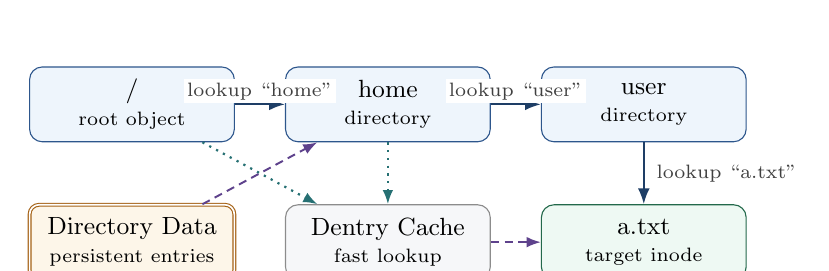
\begin{tikzpicture}[x=3.25cm,y=1.75cm]
  \node[fsnode] (root) at (0,0) {/\\[-1pt]\scriptsize root object};
  \node[fsnode] (home) at (1,0) {home\\[-1pt]\scriptsize directory};
  \node[fsnode] (user) at (2,0) {user\\[-1pt]\scriptsize directory};
  \node[fsnodeg] (file) at (2,-1) {a.txt\\[-1pt]\scriptsize target inode};
  \node[fsnodegray] (dcache) at (1,-1) {Dentry Cache\\[-1pt]\scriptsize fast lookup};
  \node[persist] (dir) at (0,-1) {Directory Data\\[-1pt]\scriptsize persistent entries};
  \draw[mainflow] (root) -- node[labelnote,above]{lookup ``home''} (home);
  \draw[mainflow] (home) -- node[labelnote,above]{lookup ``user''} (user);
  \draw[mainflow] (user) -- node[labelnote,right=3pt]{lookup ``a.txt''} (file);
  \draw[optedge] (root) -- (dcache);
  \draw[optedge] (home) -- (dcache);
  \draw[refedge] (dcache) -- (file);
  \draw[refedge] (dir) -- (home);
\end{tikzpicture}
\captionof{figure}{路径解析：先沿目录逐级推进，dcache 是可选 快路径，而不是磁盘目录项本身。}
\end{center}

\subsection{绝对路径、相对路径与搜索起点}
\begin{itemize}
  \item 绝对路径通常从进程可见的 root 开始；
  \item 相对路径从 current working directory 开始；
  \item \code{openat()} 一类接口允许把“起点目录”显式变成一个目录 fd，从而减少对全局 cwd 的依赖并避免部分 pathname race。
\end{itemize}

\subsection{硬链接：多个名字，同一个对象}
\[
\text{name}_1\dashrightarrow I_X \dashleftarrow\text{name}_2.
\]
核心结论：
\begin{itemize}
  \item 两个名字地位对等；
  \item 创建硬链接增加对象的 link count；
  \item 删除一个目录项只删除一条命名边；
  \item 通常不能跨文件系统，因为 inode number/对象身份属于具体文件系统；
  \item 普通用户通常不能随意为目录建立硬链接，以免命名空间产生复杂环路。
\end{itemize}

\subsection{符号链接：一个独立对象，内容解释为路径}
符号链接本身有自己的文件对象/元数据，其内容语义上是目标 pathname。路径解析遇到 symlink 时，会根据规则继续解析目标路径，因此：
\begin{itemize}
  \item 可跨文件系统；
  \item 可指向目录；
  \item 目标删除后 symlink 仍存在，但可能变成 dangling link；
  \item 它增加的是“路径解释层”，不是目标 inode 的 link count。
\end{itemize}

\section{第 3 章：VFS 与 Mount——把多个文件系统拼成一个命名空间}

\subsection{为什么需要 VFS}
如果每种文件系统都让应用调用不同 API，那么 \code{open/read/write/stat} 无法成为统一接口。VFS 的作用是：
\[
\boxed{\text{Common filesystem API}\arr\text{polymorphic filesystem operations}}
\]
它既向用户空间提供统一文件接口，也在内核中允许 ext4、tmpfs、NFS 等不同实现共存。

\subsection{VFS 四类核心对象的职责}
\begin{center}
\small
\begin{tabularx}{\linewidth}{>{\bfseries}p{0.18\linewidth} X X}
\toprule
对象 & 回答的问题 & 稳定心智模型 \\
\midrule
superblock & 这是哪个已挂载文件系统实例？ & 文件系统级状态/操作集合 \\
inode & 这个文件系统对象是谁？ & 元数据、权限、对象级操作 \\
dentry & 这个名字组件当前解析到谁？ & 内存 pathname cache/object binding \\
file & 这一次打开实例怎样访问对象？ & offset、status flags、访问操作 \\
\bottomrule
\end{tabularx}
\end{center}

\begin{center}
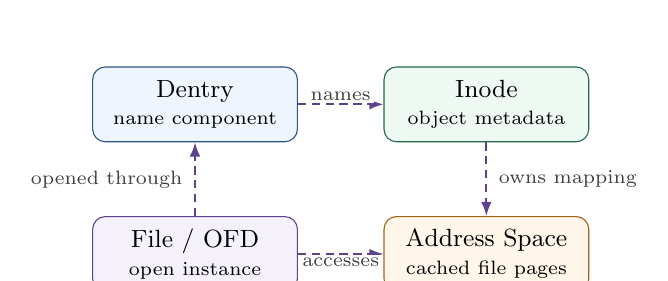
\begin{tikzpicture}[x=3.7cm,y=1.9cm]
  \node[fsnode] (dentry) at (0,0) {Dentry\\[-1pt]\scriptsize name component};
  \node[fsnodeg] (inode) at (1,0) {Inode\\[-1pt]\scriptsize object metadata};
  \node[fsnodep] (file) at (0,-1) {File / OFD\\[-1pt]\scriptsize open instance};
  \node[fsnodeo] (mapping) at (1,-1) {Address Space\\[-1pt]\scriptsize cached file pages};
  \draw[refedge] (dentry) -- node[labelnote,above]{names} (inode);
  \draw[refedge] (file) -- node[labelnote,left=3pt]{opened through} (dentry);
  \draw[refedge] (file) -- node[labelnote,below]{accesses} (mapping);
  \draw[refedge] (inode) -- node[labelnote,right=3pt]{owns mapping} (mapping);
\end{tikzpicture}
\captionof{figure}{VFS 四对象：图中虚线统一表示“引用/关联”，不与动态控制流混淆。}
\end{center}

\subsection{Mount 的本质：命名空间边界跳转}
挂载不是“把磁盘内容复制进目录”，而是让 pathname walk 到达某个 mount point 时，\kw{切换到另一个文件系统实例的根对象}。因此：
\[
\boxed{\text{one namespace tree}\neq\text{one physical filesystem}}
\]
同一路径树可以跨越多个 superblock/文件系统实例。

\begin{exam}[考试范围边界]
408 常见范围包括文件元数据与 inode、文件操作、文件保护、逻辑/物理结构、目录、硬/软链接、文件系统全局布局、空闲空间管理、VFS 与挂载。Journaling、extents、dcache/XArray 用于深化机制或说明工程边界，不替代教材模型。
\end{exam}

\section{Part II：进程怎样引用已经找到的文件}

\section{第 4 章：fd、打开文件描述与 inode}

\subsection{为什么不能让 fd 直接等于 inode}
如果 \code{fd} 直接指向 inode，那么同一文件被独立打开两次时，两个访问者如何拥有独立 offset？\code{O_APPEND} 等“打开实例状态”又放哪里？

于是必须增加一层：
\[
\boxed{\text{fd}\arr\text{打开文件描述（OFD）}\arr\text{inode}}
\]
POSIX 语义中，每次成功 \code{open()} 创建一个新的打开文件描述（open file description，OFD）；文件 offset 和 file status flags 属于它，而 fd 只是进程内的句柄。

\subsection{三种最重要的共享关系}
\begin{center}
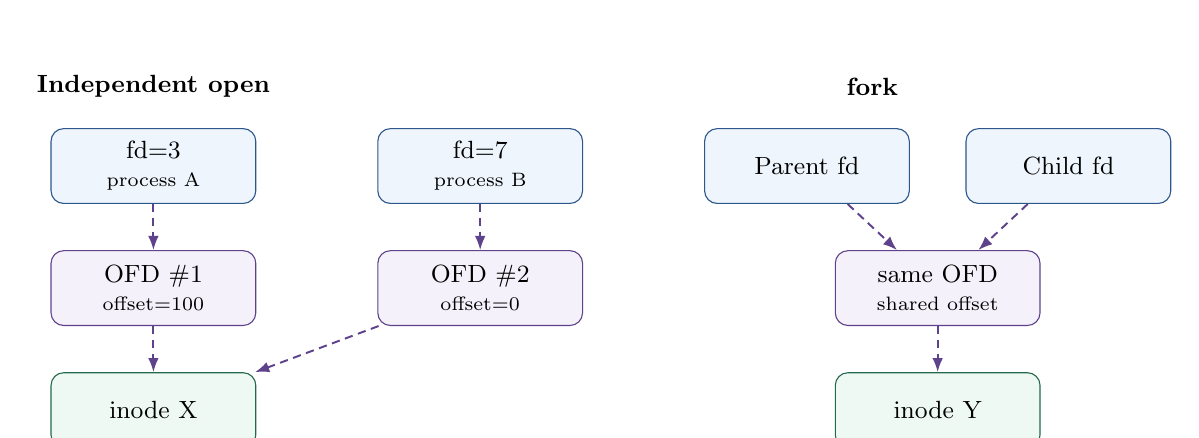
\begin{tikzpicture}[x=4.15cm,y=1.55cm]
  % independent
  \node[font=\small\bfseries] at (0,0.65) {Independent open};
  \node[fsnode] (a1) at (0,0) {fd=3\\[-1pt]\scriptsize process A};
  \node[fsnodep] (a2) at (0,-1) {OFD \#1\\[-1pt]\scriptsize offset=100};
  \node[fsnodeg] (ai) at (0,-2) {inode X};
  \draw[refedge] (a1) -- (a2); \draw[refedge] (a2) -- (ai);
  \node[fsnode] (b1) at (1,0) {fd=7\\[-1pt]\scriptsize process B};
  \node[fsnodep] (b2) at (1,-1) {OFD \#2\\[-1pt]\scriptsize offset=0};
  \draw[refedge] (b1) -- (b2); \draw[refedge] (b2) -- (ai);
  % fork
  \node[font=\small\bfseries] at (2.2,0.65) {fork};
  \node[fsnode] (pfd) at (2.0,0) {Parent fd};
  \node[fsnode] (cfd) at (2.8,0) {Child fd};
  \node[fsnodep] (fofd) at (2.4,-1) {same OFD\\[-1pt]\scriptsize shared offset};
  \node[fsnodeg] (fi) at (2.4,-2) {inode Y};
  \draw[refedge] (pfd) -- (fofd); \draw[refedge] (cfd) -- (fofd); \draw[refedge] (fofd) -- (fi);
\end{tikzpicture}
\captionof{figure}{独立 open 产生独立 OFD；fork 后对应 fd 引用同一 OFD，因此共享 file offset。}
\end{center}

\begin{center}
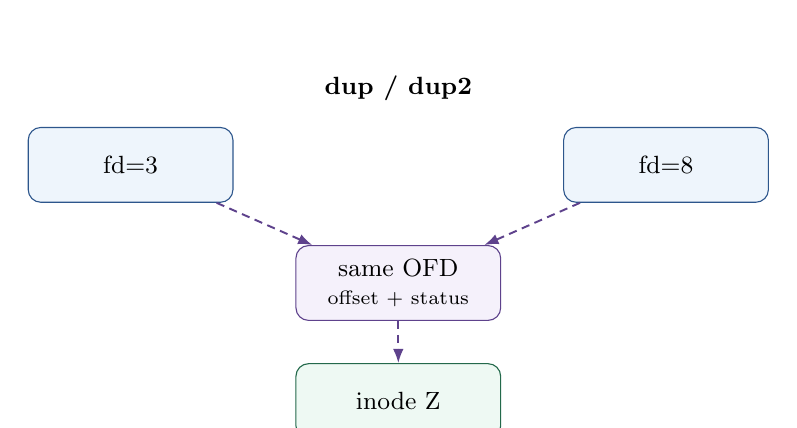
\begin{tikzpicture}[x=3.4cm,y=1.5cm]
  \node[font=\small\bfseries] at (1,0.65) {dup / dup2};
  \node[fsnode] (fd3) at (0,0) {fd=3};
  \node[fsnode] (fd8) at (2,0) {fd=8};
  \node[fsnodep] (ofd) at (1,-1) {same OFD\\[-1pt]\scriptsize offset + status};
  \node[fsnodeg] (inode) at (1,-2) {inode Z};
  \draw[refedge] (fd3) -- (ofd);
  \draw[refedge] (fd8) -- (ofd);
  \draw[refedge] (ofd) -- (inode);
\end{tikzpicture}
\captionof{figure}{dup 不会再次 open，而是增加一个 fd 句柄指向同一个 OFD。}
\end{center}

\subsection{一个稳定的题目判断法}
遇到“offset 是否共享”时，不要背父子/进程关系，直接问：
\[
\boxed{\text{Do these descriptors refer to the same OFD?}}
\]
\begin{itemize}
  \item 独立 \code{open()}：通常不同 OFD，offset 独立；
  \item \code{dup/dup2()}：同一 OFD，offset 共享；
  \item \code{fork()}：子进程 fd 与父进程对应 fd 指向同一 OFD，offset 共享；
  \item \code{exec()}：不是创建新进程；未被 close-on-exec 关闭的 fd 可继续存在。
\end{itemize}

\begin{warn}[不要把“系统级打开文件表”想成“每个文件只有一个表项”]
一个 inode 可以同时被多个 OFD 引用。\kw{文件对象身份}和\kw{打开实例状态}必须分开，否则无法解释“同一文件独立打开两次 offset 不共享”。
\end{warn}

\section{第 5 章：文件生命周期——名字引用与打开引用是两套生命线}

\subsection{unlink 删除的首先是一条命名边}
POSIX \code{unlink()} 的稳定语义是：删除 directory entry/link 并递减 link count。若最后一个 link 已删除但仍有打开引用，文件内容的最终回收要推迟到这些引用关闭。

\begin{center}
\begin{tikzpicture}[x=3.45cm,y=1.55cm]
  \node[fsnode] (name) at (0,0) {Name\\[-1pt]\scriptsize a.txt};
  \node[fsnodeg] (inode) at (1,0) {inode X\\[-1pt]\scriptsize nlink=1};
  \node[fsnodep] (ofd) at (2,0) {Open File\\[-1pt]\scriptsize still referenced};
  \node[fsnode] (fd) at (3,0) {fd=3};
  \draw[refedge] (name) -- (inode);
  \draw[refedge] (ofd) -- (inode);
  \draw[refedge] (fd) -- (ofd);
  \draw[crossout] ($(name.east)!0.45!(inode.west)+(0,0.18)$) -- ($(name.east)!0.55!(inode.west)+(0,-0.18)$);
  \draw[crossout] ($(name.east)!0.45!(inode.west)+(0,-0.18)$) -- ($(name.east)!0.55!(inode.west)+(0,0.18)$);
  \node[labelnote] at (0.5,-0.42) {unlink 删除 name$\to$object};
\end{tikzpicture}
\captionof{figure}{unlink while open：名字可以消失，而已经建立的打开引用继续访问同一对象。}
\end{center}

\subsection{双生命周期模型}
\begin{itemize}
  \item \kw{Name lifetime}：有多少持久目录链接仍指向对象？（经典 UNIX 用 link count 表达）
  \item \kw{打开引用生命周期}：运行时是否仍有 OFD 或其他内核引用使对象继续存活？
\end{itemize}
真正安全的高层结论是：
\[
\boxed{\text{no persistent names} + \text{no live references} \Rightarrow \text{eligible for final reclamation}}
\]

\begin{eng}[Linux 实现边界]
不要把教材中的“打开计数”机械等同于 Linux \code{inode.i_count}。\code{struct file}、inode cache、dentry cache 都有各自引用/回收机制。408 做题时可以用“链接引用 + 打开引用”两类计数理解生命周期；工程实现则更细。
\end{eng}

\subsection{create、link、unlink、rename 分别改什么}
\begin{center}
\small
\begin{tabularx}{\linewidth}{>{\bfseries}p{0.16\linewidth} X X}
\toprule
操作 & 命名空间变化 & 对象/元数据变化 \\
\midrule
create & 新增 name $\to$ new object & 分配/初始化对象元数据，通常 link count 从 1 开始 \\
link & 新增 second name $\to$ same object & link count 增加 \\
unlink & 删除一条 name $\to$ object & link count 减少；是否最终回收看剩余引用 \\
rename & 把名字关系从旧位置移动/替换到新位置 & 通常不改变文件内容本身，重点是目录元数据的一致更新 \\
\bottomrule
\end{tabularx}
\end{center}

\section{第 6 章：文件保护——谁可以对哪个对象做什么}
文件保护的统一问题是：
\[
\boxed{\text{Subject}\times\text{Object}\times\text{Operation}\to\{allow,deny\}}
\]
408 常见机制包括访问权限，以及所有者、所属组、其他用户的读写执行位。目录的读、写、执行权限与普通文件语义不同：目录执行权限表示允许搜索或穿越，写权限与创建、删除目录项相关。

\begin{method}[保护题三问]
\begin{enumerate}
  \item 当前 subject 是谁（用户/进程/权限域）？
  \item 当前 object 是普通文件还是目录？
  \item 请求 operation 是读取内容、修改内容、创建名字、删除名字还是穿越目录？
\end{enumerate}
不要只看到“rwx”就机械对应同一含义。
\end{method}

\section{Part III：文件中的字节怎样落到块上}

\section{第 7 章：从文件偏移到逻辑块}
设文件系统块大小为 $B$，字节偏移为 $x$：
\[
\boxed{LBN=\left\lfloor\frac{x}{B}\right\rfloor},\qquad
\boxed{off_{in}=x\bmod B}.
\]
这一步只把\kw{文件内部字节位置}转换成\kw{文件内部逻辑块号}，还没有决定它在磁盘哪个位置。

\begin{warn}[三个“地址”不要混]
\begin{itemize}
  \item File offset：文件内的字节序号；
  \item LBN：文件自己的逻辑块号；
  \item filesystem block / device location：底层存储位置。
\end{itemize}
它们对应的层次不同，不能把 \code{offset/B} 的结果直接叫“磁盘块号”。
\end{warn}

\section{第 8 章：文件物理结构——三种经典方案从矛盾中产生}

\subsection{连续分配：数组模型}
若文件占据连续块区间：
\[
PBN = start + LBN.
\]
\kw{优点}：随机与顺序访问都直接，局部性好。\kw{代价}：增长困难、外部碎片、预估大小困难。

\subsection{链接分配：链表模型}
每个数据块保存“下一块”的位置：
\[
B_0\to B_7\to B_{19}\to\cdots
\]
\kw{优点}：增长灵活、没有经典外部碎片问题。\kw{代价}：隐式链随机访问差，指针损坏影响链后部。

\paragraph{FAT：把链从数据块搬进集中表}
FAT 把“下一簇号”集中存储，使链遍历可在内存 FAT 中进行；因此它仍是 linked allocation 思想，但显著改善了定位开销（在 FAT 已在内存的题设下）。

\subsection{索引分配：映射表模型}
把数据块地址集中放进索引结构：
\[
LBN\xrightarrow{index}PBN.
\]
它和页表有明显同构：都通过增加一层 indirection，换来离散布局、随机定位和灵活增长。

\begin{bridge}[VM 与 File System 的共同设计语言]
\[
\text{VPN}\to\text{Page Table}\to\text{PFN}
\]
和
\[
\text{LBN}\to\text{File Index}\to\text{Storage Block}
\]
本质都是“逻辑编号 $\to$ 映射结构 $\to$ 物理位置”。系统设计反复用\kw{间接层}换取 relocation、sharing、sparse allocation 与 growth flexibility。
\end{bridge}

\section{第 9 章：inode 多级索引——408 计算题的统一模型}

\subsection{经典 UNIX-style mixed indexing}
设一个 inode 中有：
\begin{itemize}
  \item $d$ 个直接指针；
  \item $s$ 个一级间接指针；
  \item $q$ 个二级间接指针；
  \item $t$ 个三级间接指针。
\end{itemize}
文件系统块大小为 $B$，块地址项大小为 $a$，则一个索引块可容纳：
\[
\boxed{K=\left\lfloor\frac{B}{a}\right\rfloor}
\]
个地址项。

最大可寻址数据块数：
\[
\boxed{N_{max}=d+sK+qK^2+tK^3}
\]
最大文件大小：
\[
\boxed{Size_{max}=N_{max}\cdot B}.
\]

\begin{center}
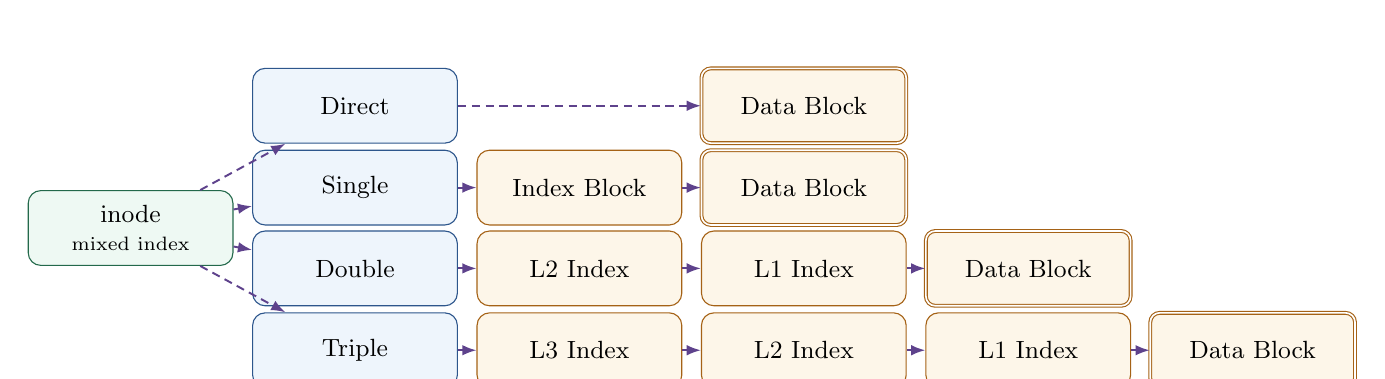
\begin{tikzpicture}[x=2.85cm,y=1.35cm]
  \node[fsnodeg] (ino) at (0,0) {inode\\[-1pt]\scriptsize mixed index};
  \node[fsnode] (d) at (1,1.15) {Direct};
  \node[fsnode] (s) at (1,0.38) {Single};
  \node[fsnode] (q) at (1,-0.38) {Double};
  \node[fsnode] (t) at (1,-1.15) {Triple};
  \node[persist] (bd) at (3,1.15) {Data Block};
  \node[fsnodeo] (i1) at (2,0.38) {Index Block};
  \node[fsnodeo] (i2a) at (2,-0.38) {L2 Index};
  \node[fsnodeo] (i2b) at (3,-0.38) {L1 Index};
  \node[fsnodeo] (i3a) at (2,-1.15) {L3 Index};
  \node[fsnodeo] (i3b) at (3,-1.15) {L2 Index};
  \node[fsnodeo] (i3c) at (4,-1.15) {L1 Index};
  \node[persist] (bs) at (3,0.38) {Data Block};
  \node[persist] (bq) at (4,-0.38) {Data Block};
  \node[persist] (bt) at (5,-1.15) {Data Block};
  \draw[refedge] (ino) -- (d); \draw[refedge] (ino) -- (s); \draw[refedge] (ino) -- (q); \draw[refedge] (ino) -- (t);
  \draw[refedge] (d) -- (bd);
  \draw[refedge] (s) -- (i1); \draw[refedge] (i1) -- (bs);
  \draw[refedge] (q) -- (i2a); \draw[refedge] (i2a) -- (i2b); \draw[refedge] (i2b) -- (bq);
  \draw[refedge] (t) -- (i3a); \draw[refedge] (i3a) -- (i3b); \draw[refedge] (i3b) -- (i3c); \draw[refedge] (i3c) -- (bt);
\end{tikzpicture}
\captionof{figure}{经典 inode 混合索引。每增加一级间接，就多一次索引块解析机会与空间层级。}
\end{center}

\subsection{I/O 次数一定先写缓存假设}
典型题设“inode 已在内存、相关索引块均未缓存”：
\begin{itemize}
  \item 直接块：读数据需要 1 次块 I/O；
  \item 一级间接：索引块 + 数据块，共 2 次；
  \item 二级间接：两级索引 + 数据，共 3 次；
  \item 三级间接：三级索引 + 数据，共 4 次。
\end{itemize}
但如果索引块已缓存，次数会下降。因此任何 I/O 计算都先写：\kw{inode 是否在内存？索引块是否缓存？目录块是否缓存？页缓存 是否命中？}

\begin{eng}[现代 ext4：extent 不是“12+1+1+1”的简单延长]
经典 direct/single/double/triple 模型非常适合 408 计算题；现代 ext4 可使用 extent tree，把“连续逻辑范围 $\to$ 连续物理范围”作为映射单位。Linux ext4 文档明确区分 inode 的 extent 格式等结构。工程边界用于理解“现代文件系统为何减少大文件映射元数据”，但不替代经典计算模型。
\end{eng}

\section{Part IV：空间从哪里来——Global Layout 与 Free Space}

\section{第 10 章：文件系统全局 Layout}

\subsection{为什么必须有全局账本}
文件系统不能只存“每个文件的 inode”。它还必须知道：
\begin{itemize}
  \item 文件系统总大小与块大小；
  \item 哪些 inode/数据块空闲；
  \item inode table 在哪里；
  \item 根对象与挂载状态；
  \item 日志、特性标志、校验信息等。
\end{itemize}
因此出现 superblock、bitmap、inode table、data region 等全局结构。

\begin{center}
\small
\begin{tabularx}{\linewidth}{>{\bfseries}p{0.18\linewidth} X X}
\toprule
结构 & 解决的问题 & 典型信息 \\
\midrule
Superblock & 这个文件系统实例整体是什么？ & block size、总量、特性、状态等 \\
Inode bitmap & 哪些 inode identity 可分配？ & 每个 inode 的 free/used 状态 \\
Block bitmap & 哪些 data/fs blocks 可分配？ & 每块 free/used 状态 \\
Inode table & 每个对象元数据持久放在哪里？ & inode records \\
Data region & 文件/目录的内容在哪里？ & data blocks / index / extents \\
Journal（扩展） & 多结构更新如何恢复？ & transaction records / commit \\
\bottomrule
\end{tabularx}
\end{center}

\begin{eng}[ext4 block groups]
现代 ext4 会把磁盘划成 block groups，并在组内组织 bitmap、inode table 与数据块，以提高局部性并减少碎片/寻道成本。它说明一个更普遍的设计原则：\kw{空间分配不仅追求“能分到”，还追求 metadata 与 data 的局部性。}
\end{eng}

\section{第 11 章：外存空闲空间管理}

\subsection{位图 Bitmap}
用 1 bit 表示一个单位是否空闲。优点是结构紧凑，寻找连续空闲范围和统计较方便；代价是需要扫描/维护位图并保持一致性。

\subsection{空闲链表 Free List}
把空闲块串起来。结构简单，但想找一段连续空间或一次分配很多块时可能遍历成本高。

\subsection{成组链接 Grouped Linking}
把若干空闲块号作为一组集中保存，再用某个块连接下一组。经典 UNIX 教学模型用它降低频繁访问长链的成本。

\subsection{计数法 Counting}
当空闲块经常成片连续时，用：
\[
(start, count)
\]
记录一段空闲区。它体现一个普遍优化：\kw{不要逐块记录具有强连续性的状态，而要记录范围。}

\begin{exam}[空闲空间题不要只问“哪个方法快”]
固定四问：\kw{元数据多大？找一个块快不快？找连续 $k$ 块快不快？回收/合并是否方便？} 不同 workload 下不存在绝对最好方案。
\end{exam}

\section{Part V：文件操作怎样真正运行}

\section{第 12 章：一次 open() 的一生}

\subsection{open 的高层语义}
\code{open(path, flags)} 不是“把文件内容读进来”，而是建立：
\[
\boxed{\text{pathname}\arr\text{object}\arr\text{new OFD}\arr\text{fd}}
\]
其中 \code{open()} 的 POSIX 语义包括创建新的 OFD，并让一个 fd 指向它；常规文件初始 offset 通常从文件开头开始（特定 flag 另行处理）。

\begin{center}
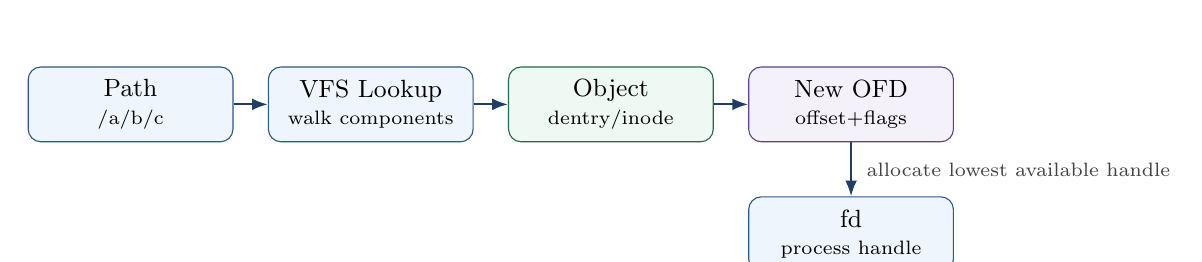
\begin{tikzpicture}[x=3.05cm,y=1.65cm]
  \node[fsnode] (path) at (0,0) {Path\\[-1pt]\scriptsize /a/b/c};
  \node[fsnode] (lookup) at (1,0) {VFS Lookup\\[-1pt]\scriptsize walk components};
  \node[fsnodeg] (inode) at (2,0) {Object\\[-1pt]\scriptsize dentry/inode};
  \node[fsnodep] (ofd) at (3,0) {New OFD\\[-1pt]\scriptsize offset+flags};
  \node[fsnode] (fd) at (3,-1) {fd\\[-1pt]\scriptsize process handle};
  \draw[mainflow] (path) -- (lookup);
  \draw[mainflow] (lookup) -- (inode);
  \draw[mainflow] (inode) -- (ofd);
  \draw[mainflow] (ofd) -- node[labelnote,right=4pt]{allocate lowest available handle} (fd);
\end{tikzpicture}
\captionof{figure}{open() 的核心不是读数据，而是把“名字”转成“运行时访问关系”。}
\end{center}

\subsection{open 题型的状态跟踪}
\begin{enumerate}
  \item 路径从哪个起点解析？绝对、cwd 还是 dirfd？
  \item 每个 component 是否命中 dcache？如果题目按磁盘 I/O 计数，需要哪些目录块/inode？
  \item 最终对象权限是否允许请求模式？
  \item 是 independent open 还是已有 fd 的 dup/fork 共享？
  \item 返回的 fd 是否按题设采用“最小可用非负整数”？
\end{enumerate}

\section{第 13 章：一次 read(fd, buf, n) 的文件系统路径}

\subsection{先定位打开实例，再定位文件位置}
\[
fd\arr OFD\arr\{offset,flags,object\}.
\]
随后根据 offset 计算文件页/逻辑块位置。

\subsection{现代 buffered read：先问 页缓存}
普通 buffered file I/O 中，更合理的逻辑是：
\[
\boxed{(file,page\ index)\arr Page\ Cache?}
\]
而不是先无条件算 PBN 再查缓存。若命中，直接从缓存页向用户缓冲提供数据；若未命中，具体文件系统才需要建立文件偏移到存储位置的映射并向 I/O 子系统提交读取。

\begin{center}
\begin{tikzpicture}[x=3.0cm,y=1.55cm]
  \node[fsnode] (fd) at (0,0) {fd};
  \node[fsnodep] (ofd) at (1,0) {OFD\\[-1pt]\scriptsize current offset};
  \node[fsnodeg] (inode) at (2,0) {inode/file};
  \node[fsnode] (pc) at (3,0) {页缓存?};
  \node[fsnodeg] (hit) at (3,-1) {Hit\\[-1pt]\scriptsize copy to user};
  \node[fsnodeo] (miss) at (2,-1) {Miss\\[-1pt]\scriptsize block mapping};
  \node[fsnodegray] (io) at (1,-1) {I/O System\\[-1pt]\scriptsize submit request};
  \draw[mainflow] (fd) -- (ofd); \draw[mainflow] (ofd) -- (inode); \draw[mainflow] (inode) -- (pc);
  \draw[mainflow] (pc) -- node[labelnote,right=3pt]{快路径} (hit);
  \draw[mainflow] (pc) -- (miss); \draw[mainflow] (miss) -- (io);
\end{tikzpicture}
\captionof{figure}{read() 的文件系统边界：到 I/O request 为止；DMA/interrupt/wakeup 已由 I/O 专题负责。}
\end{center}

\subsection{跨块读取}
如果读取范围跨多个文件页/块，不能只计算起始 LBN：
\[
LBN_{start}=\left\lfloor\frac{off}{B}\right\rfloor,
\quad
LBN_{end}=\left\lfloor\frac{off+n-1}{B}\right\rfloor.
\]
实际读取字节数还受到 EOF 限制。

\section{第 14 章：一次 write(fd, buf, n) 的文件系统路径}

\subsection{Buffered write 的核心状态变化}
常见普通写路径：
\[
\text{User Data}\arr\text{页缓存}\arr\text{Dirty}
\]
并更新文件 offset、size/mtime 等相关内存元数据。系统调用返回与“数据已经稳定落盘”不是同一时间点。

\begin{bridge}[与 I/O 专题接口]
本册只追到：\kw{dirty cached pages + block mapping + writeback request}。请求提交以后，设备队列、driver、DMA、completion interrupt 等交给 I/O 专题。这样两册之间只有接口，不重复整条设备路径。
\end{bridge}

\subsection{写入可能同时修改哪些状态}
\begin{itemize}
  \item 文件数据页；
  \item file size（若扩展）；
  \item mtime/ctime 等元数据；
  \item block allocation metadata（若需要新块）；
  \item block mapping/index/extent；
  \item OFD 的 offset。
\end{itemize}
正因为一次高层 \code{write} 可能对应多份持久结构更新，后面才会产生 crash consistency 问题。

\section{第 15 章：create、close、unlink、rename 的状态机}

\subsection{create：先创造身份，再绑定名字}
以经典 inode 模型看，新建文件至少需要：
\begin{enumerate}
  \item 找到父目录；
  \item 分配对象身份/inode；
  \item 初始化 metadata；
  \item 在父目录中建立 name $\to$ inode 映射；
  \item 若同时打开，再创建 OFD 与 fd。
\end{enumerate}
创建空文件时不必立刻拥有数据块；实际数据块可在后续写入时按需分配。你原有材料把“inode bitmap、inode table、parent directory”识别为核心持久结构，这是理解 crash consistency 的好入口。

\subsection{close：释放一个 handle，不等于删除文件}
\code{close(fd)} 首先终止当前 fd 对 OFD 的引用。只有当相应运行时引用都消失，OFD 才可回收；而持久文件是否存在仍由命名空间链接等状态决定。

\subsection{rename：名字变化不等于内容复制}
高层语义重点是对 namespace 的原子式名称变更/替换要求，而不是“把全部数据重新写一遍”。这也是为什么 rename 常被应用用作构造持久更新协议的一部分，但具体持久化保证仍要结合文件系统与同步调用分析。

\section{Part VI：为什么“写完”以后文件系统仍可能坏}

\section{第 16 章：Crash Consistency——持久状态机的核心问题}

\subsection{高层一次操作，底层多次写}
假设 append/create 需要更新：
\[
W_1=\text{bitmap},\quad W_2=\text{inode},\quad W_3=\text{directory/data}.
\]
设备只能在时间上逐步持久化它们，崩溃可以发生在任意两步之间。因此我们要的是：
\[
\boxed{\text{after reboot, on-disk state must correspond to a legal filesystem state}}
\]
而不是假设“一次系统调用天然就是一次原子磁盘事务”。

\begin{center}
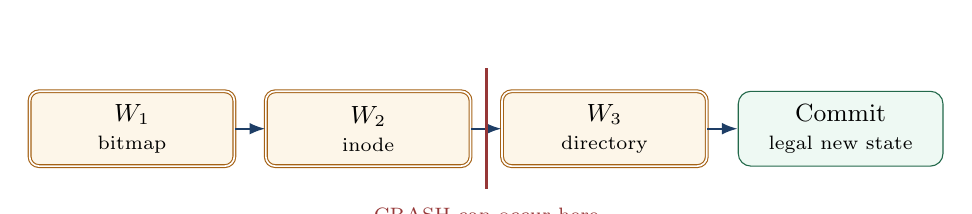
\begin{tikzpicture}[x=3.0cm,y=1.4cm]
  \node[persist] (w1) at (0,0) {$W_1$\\[-1pt]\scriptsize bitmap};
  \node[persist] (w2) at (1,0) {$W_2$\\[-1pt]\scriptsize inode};
  \node[persist] (w3) at (2,0) {$W_3$\\[-1pt]\scriptsize directory};
  \node[fsnodeg] (commit) at (3,0) {Commit\\[-1pt]\scriptsize legal new state};
  \draw[mainflow] (w1) -- (w2); \draw[mainflow] (w2) -- (w3); \draw[mainflow] (w3) -- (commit);
  \draw[deepred,line width=1.2pt] (1.5,0.55) -- (1.5,-0.55);
  \node[labelnote,text=deepred] at (1.5,-0.78) {CRASH can occur here};
\end{tikzpicture}
\captionof{figure}{Crash consistency 的数学对象不是单个写，而是“多写序列 + 任意崩溃点”。}
\end{center}

\subsection{崩溃分析五步法}
\begin{method}[Crash Point Analysis]
\begin{enumerate}
  \item 列出高层操作会修改的所有持久对象；
  \item 写出允许/要求的持久化顺序；
  \item 标出 commit point 或“完成”的判据；
  \item 在每两次持久写之间插入 crash；
  \item 对每个 crash state 问：哪些结构互相矛盾？重启后是 ignore、redo、undo 还是 repair？
\end{enumerate}
\end{method}

\section{第 17 章：fsck 与 Journaling}

\subsection{fsck：允许不一致，重启后扫描修复}
早期思路可以概括为：正常运行不维护完整事务日志，crash 后遍历 inode、bitmap、目录等结构，检查引用数、空间使用与对象关系是否自洽，再修复。

优势：运行时机制简单。代价：大文件系统全盘检查慢，而且“修复到一致”不一定等价于恢复用户最期望的最近状态。

\subsection{Journaling：先记录一笔可重放的事务}
经典 write-ahead logging 思路：
\[
\boxed{\text{Log Records}\arr\text{Commit}\arr\text{Checkpoint/Home Locations}}
\]
只有看到有效 commit 的事务才视为已提交；重启时可以根据日志 replay 已提交但尚未 checkpoint 完成的修改。

\begin{eng}[工程边界：ext4/JBD2]
ext4 使用 jbd2 journal 保护文件系统免于元数据更新中途崩溃造成结构不一致。官方文档说明：事务完整写入并有 commit record 后，可在恢复时 replay；默认 \code{data=ordered} 模式主要 journal metadata，并要求相关 data 在 metadata commit 前按规则写出。\kw{这是一种现代实现实例，不应替代 408 对 journaling/WAL 一般机制的理解。}
\end{eng}

\subsection{Consistency 与 Durability 不完全是一件事}
\begin{itemize}
  \item \kw{Consistency}：磁盘上的结构彼此不矛盾、符合文件系统不变量；
  \item \kw{Durability/Freshness}：应用刚写的数据到底已经持久到什么程度。
\end{itemize}
文件系统可以在 crash 后结构一致，但丢失最近尚未达到持久边界的数据。因此 \code{write()} 返回、后台 writeback、journal commit、\code{fsync()} 完成、设备 cache flush 是不同层次的时间点。

\section{Part VII：408 计算与解题工具箱}

\section{第 18 章：经典计算模型}

\subsection{模型 A：最大文件大小}
步骤：
\begin{enumerate}
  \item 求索引块地址项数 $K=B/a$；
  \item 分别计算 direct、single、double、triple 能覆盖的数据块数；
  \item 相加后乘块大小；
  \item 检查题目是否还有 inode 本身大小、最大文件长度字段、编号位宽等额外限制。
\end{enumerate}

\subsection{模型 B：判断目标字节属于哪一级索引}
先：
\[
LBN=\left\lfloor\frac{x}{B}\right\rfloor.
\]
再与区间比较：
\[
[0,d),\quad[d,d+sK),\quad[d+sK,d+sK+qK^2),\ldots
\]
确定索引级别，然后计算对应索引项序号。

\subsection{模型 C：磁盘 I/O 次数}
任何次数题先写假设表：
\begin{center}
\small
\begin{tabularx}{\linewidth}{>{\bfseries}p{0.26\linewidth} X}
\toprule
对象 & 题设状态 \\
\midrule
目录块/dentry & 在内存？需要逐级读盘？ \\
inode & 已在内存？ \\
间接索引块 & 已缓存？ \\
数据页/页缓存 & hit 还是 miss？ \\
FAT & 是否假设常驻内存？ \\
写回 & 题目只算逻辑读取，还是连 metadata/writeback 都算？ \\
\bottomrule
\end{tabularx}
\end{center}
不写这些前提就直接报一个 I/O 次数，通常是不严谨的。

\subsection{模型 D：路径查找 I/O}
不要机械说 \code{/a/b/c} 就一定 3 次或 6 次。路径解析可能涉及每一级目录 inode、目录数据块以及目标 inode；缓存与题设会极大改变次数。正确方法是画访问序列，再按“哪些对象已在内存”删除对应磁盘 I/O。

\section{第 19 章：高频辨析表}
\begin{center}
\small
\begin{tabularx}{\linewidth}{>{\bfseries}p{0.23\linewidth} X X}
\toprule
容易混淆 & 错误心智模型 & 正确判断 \\
\midrule
inode vs filename & inode 里面存文件名 & 名字属于目录项；inode 表示对象元数据 \\
directory entry vs dentry & 两个完全同义 & 前者可指磁盘目录记录；Linux dentry 是内存 VFS 对象 \\
fd vs inode & fd 就是文件 & fd 是进程句柄，先指向 OFD \\
OFD vs inode & 同文件只存在一个 OFD & 每次独立 open 可产生独立 OFD，共享同 inode \\
link count vs open ref & nlink=0 立刻释放数据 & 仍有打开引用时内容继续存活 \\
file offset vs PBN & offset/B 就是磁盘块 & 先得到 LBN，再经 block mapping \\
页缓存 vs block map & 先求 PBN 才能查缓存 & buffered file cache 更自然按 file mapping + page index 组织 \\
FS block vs sector & 文件系统块就是设备最小原子写 & FS block、sector、atomic write unit 是不同概念 \\
write return vs durable & write 返回就永久落盘 & buffered write、writeback、commit、durability 分层 \\
classic inode vs ext4 & ext4 就固定 12+1+1+1 & 408 经典模型保留；现代 ext4 常用 extents \\
\bottomrule
\end{tabularx}
\end{center}

\section{第 20 章：文件系统十四问——解题检查表}
\begin{method}[遇到任何文件系统题，按顺序扫描]
\begin{enumerate}
  \item 输入给的是 pathname 还是 fd？
  \item 当前操作的是名字（namespace）还是已经打开的对象？
  \item pathname 从 root、cwd 还是 dirfd 开始？
  \item 题目中的“目录项”是持久 entry 还是内存 dentry？
  \item fd 指向哪个 OFD？是否与别的 fd 共享？
  \item 当前 file offset 在哪里保存，怎样变化？
  \item byte offset 属于哪个 LBN / file page index？
  \item 页缓存 是否命中？
  \item 若需要存储访问，LBN 怎样映射到 block？
  \item 使用连续、链接/FAT、索引还是混合索引？索引块是否缓存？
  \item 是否需要分配新 inode/block？空闲空间由什么结构管理？
  \item 这次操作会修改哪些 metadata 与 data？
  \item 如果 crash 发生在任意两次持久写之间，状态是否合法？
  \item 最终题目问的是逻辑状态、生命周期、空间、I/O 次数还是持久性？
\end{enumerate}
\end{method}

\section{第 21 章：五道综合题，把整册重新跑一遍}
\subsection*{综合题 1：一个名字的一生}
\[
\texttt{/home/x/a.txt}\arr\text{component walk}\arr\text{dentry/directory lookup}\arr\text{inode/object}.
\]
训练：目录、路径、VFS、mount、link。

\subsection*{综合题 2：一次 open() 的一生}
\[
Path\arr Object\arr OFD\arr fd.
\]
训练：VFS、fd、offset、independent open/fork/dup。

\subsection*{综合题 3：一次 read() 的文件系统路径}
\[
fd\arr OFD\arr(file,offset)\arr PageCache\arr BlockMapping\arr I/O~System.
\]
训练：引用链、offset、缓存、索引计算与专题边界。

\subsection*{综合题 4：unlink 一个仍被打开的文件}
训练：Name $\neq$ Object、链接计数、打开引用与最终回收。

\subsection*{综合题 5：create/write 过程中突然 crash}
训练：bitmap、inode、directory、data 多结构更新，崩溃点分析，fsck/journaling。

\begin{corebox}[三条核心结论]
文件系统最值得记住的不是某个 inode 字段，而是三句话：
\begin{enumerate}
  \item \kw{Naming is mapping}：名字只是到对象的引用，不等于对象本身。
  \item \kw{Open is state}：打开以后必须有独立的运行时访问状态，因此 fd、OFD、inode 必须分层。
  \item \kw{Persistence is protocol}：高层一次操作会变成多个持久写，正确性来自写序、提交与恢复协议，而不是“磁盘自己不会坏”。
\end{enumerate}
\[
\boxed{\text{Name}\to\text{Object}\to\text{Open State}\to\text{Data Mapping}\to\text{Persistent Protocol}}
\]
\end{corebox}

\section{附录 A：考试模型 / 机制 / 工程边界}
\begin{center}
\footnotesize
\begin{tabularx}{\linewidth}{>{\bfseries}p{0.16\linewidth} X X X}
\toprule
主题 & 考试模型 & 机制深化 & 工程边界 \\
\midrule
文件抽象 & 文件、元数据、inode/FCB、操作、保护 & object identity、metadata/data split & VFS inode operations \\
目录 & 树形目录、路径、操作、硬/软链接 & pathname state machine & dcache、negative dentry、openat \\
打开文件 & open/close/read/write、共享 & fd$\to$OFD$\to$inode & Linux struct file/files\_struct \\
物理结构 & contiguous/linked/indexed & mixed indexing、I/O path & extents/delayed allocation \\
空间管理 & bitmap/free list/grouping 等 & locality/range allocation & ext4 block groups \\
文件系统 & layout、VFS、mounting & namespace vs filesystem instance & VFS core objects \\
持久性 & 理解写回与一致性思想 & fsck/journaling/crash points & JBD2 / ext4 data modes \\
\bottomrule
\end{tabularx}
\end{center}

\section{附录 B：参考资料与工程边界}
\begingroup\Urlmuskip=0mu plus 6mu\relax
正文以 408 教材模型为主，以下公开资料用于核对术语和工程实现边界：
\begin{itemize}
  \item Linux Kernel Documentation, \emph{Overview of the Linux Virtual File System}: \url{https://docs.kernel.org/filesystems/vfs.html}
  \item Linux Kernel Documentation, \emph{ext4 Data Structures and Algorithms}: \url{https://docs.kernel.org/filesystems/ext4/}
  \item Linux Kernel Documentation, \emph{ext4 Journal (jbd2)}: \url{https://docs.kernel.org/6.17/filesystems/ext4/journal.html}
  \item POSIX.1-2024, \code{open()}, \code{dup()}, \code{fork()}: \url{https://pubs.opengroup.org/onlinepubs/9799919799/}
  \item OSTEP, \emph{File System Implementation} 与 \emph{Crash Consistency: FSCK and Journaling}: \url{https://pages.cs.wisc.edu/~remzi/OSTEP/}
\end{itemize}
\endgroup

\end{document}
